%===========================================
%          NOTES
%===========================================
% R code to generate correlation matrix and tables is in 'Re-defining ILDs.R'

%===========================================
%          MR SUPPLEMENTARY
%===========================================
% when loading the chapter reference lists:
% run pdfLaTeX (create .aux files) + Bibtex on chapter .tex files + pdfLaTeX +pdfLaTeX  in main.tex
%\mainmatter %set numbers to arabic
%\chapter*{Mutation Relaxation (MR)}
%\vspace{-1cm}

% Changing Figures and Table names to contain 'S' ====
% this pastes 'S' to the number and thus can be used in cross references! (remember to change back if incorporated with other docs)
\subsection{Defining inter-landmark distance traits for \textit{Drosophila serrata}}

Nine landmark positions (LMs), determined by wing vein intersections (see main text Figure~\ref{fig:Fig2MetMRdsgn}), were used to characterise traits of inter-landmark distances (ILDs). Previously, wing shape in \textit{D.~serrata} has been characterised \citep{McGu15, Szte15} using ten ILD traits that were determined in \textit{D. bunnanda}, a sister species of \textit{D. serrata}, and were chosen based on wing coverage and independence (not collinear) \citep{McGu07}. However, multivariate analyses of the same set of ILD traits in \textit{D. serrata} has suffered from problems with multicollinearity (\citealp{Szte15}; \citealp{Duga21}); Aguirre \textit{et al.} unpublished). One solution to this is to simply reduce the number of traits used, eliminating highly correlated traits \citep[e.g.][]{Szte15}. However, this reduces the dimensionality of shape space that can be explored. Therefore, to remedy this problem, a new set of ILD traits were identified that allowed me to maximise the potential dimensions (traits) while eliminating the problem of collinearity. \par

All 36 combinations of ILDs from the nine wing landmarks were investigated. The final ten ILD traits were chosen, as before \citep{McGu07}, with the intent to capture independent variation in wing shape that also maximised wing coverage. To do so, three criteria were used: 1.~included traits had to vary at the genetic level, 2. included traits were not highly correlated (defined below), and 3. traits chosen resulted in good coverage of the wing space, and were not all localised to a particular region. The first criterion was imposed to ensure that zero variance of individual traits did not impede multivariate model convergence, and because the unusual pattern of no genetic (mutational) variance might indicate that traits did not capture any biological variation, only measurement error. This criterion excluded traits ILD3.4, ILD4.9, ILD6.7 and ILD8.9 (main text: Figure~\ref{fig:Fig2MetMRdsgn}; Table ~\ref{tab:CovTest}). Next, the phenotypic correlation matrix was examined (Figure~\ref{fig:CorMAt_36_ILDs}), and we excluded traits stepwise. First, trait pairs that were almost collinear (had $\rho > 0.95$) were identified and a single trait of the pair was retained. When one of the pairs was one of the \textit{D. bunnanda} ILDs previously analysed, preference was given to retain this trait; otherwise, traits were retained at random. This criterion excluded traits ILD1.7, ILD1.8, ILD2.9, ILD3.9, ILD4.6, ILD5.9, ILD6.8 and ILD7.9.\par

Next, we identified groups of traits that were highly correlated ($0.85<\rho<0.95$) because they described similar areas of wing space. For example, ILD2.5, ILD2.6 and ILD2.7 all describe wing depth, thus ILD2.5 was retained (as it was an original ILD). Similarly, landmarks were placed on both ends of the anterior and posterior cross-veins, but cross-vein length was not variable (see criterion 1), and thus ILDs depending on LM6 versus 7 or on LM8 versus 9 were highly collinear. Consequently, from ILD1.6, ILD3.6, ILD3.7, ILD4.7, ILD6.9 and ILD7.8; only ILD3.7 (original) was kept. For ILD1.2, ILD2.3, ILD2.4 and ILD2.8 all distances appear to capture the displacement of LM2 along the wing margin; ILD1.2 and ILD2.8 (original) were kept as they had the lowest correlation coefficients and were capturing other parts of the wing shape. From the remaining 15 wing ILD traits that had correlation coefficients $\leq 0.8$, the final 10 traits were picked to ensure entire wing shape coverage, utilising all nine landmarks.\par

%\newpage

%% ========Classic Nine Wing Landmarks=============
%\begin{figure}[hbp]
%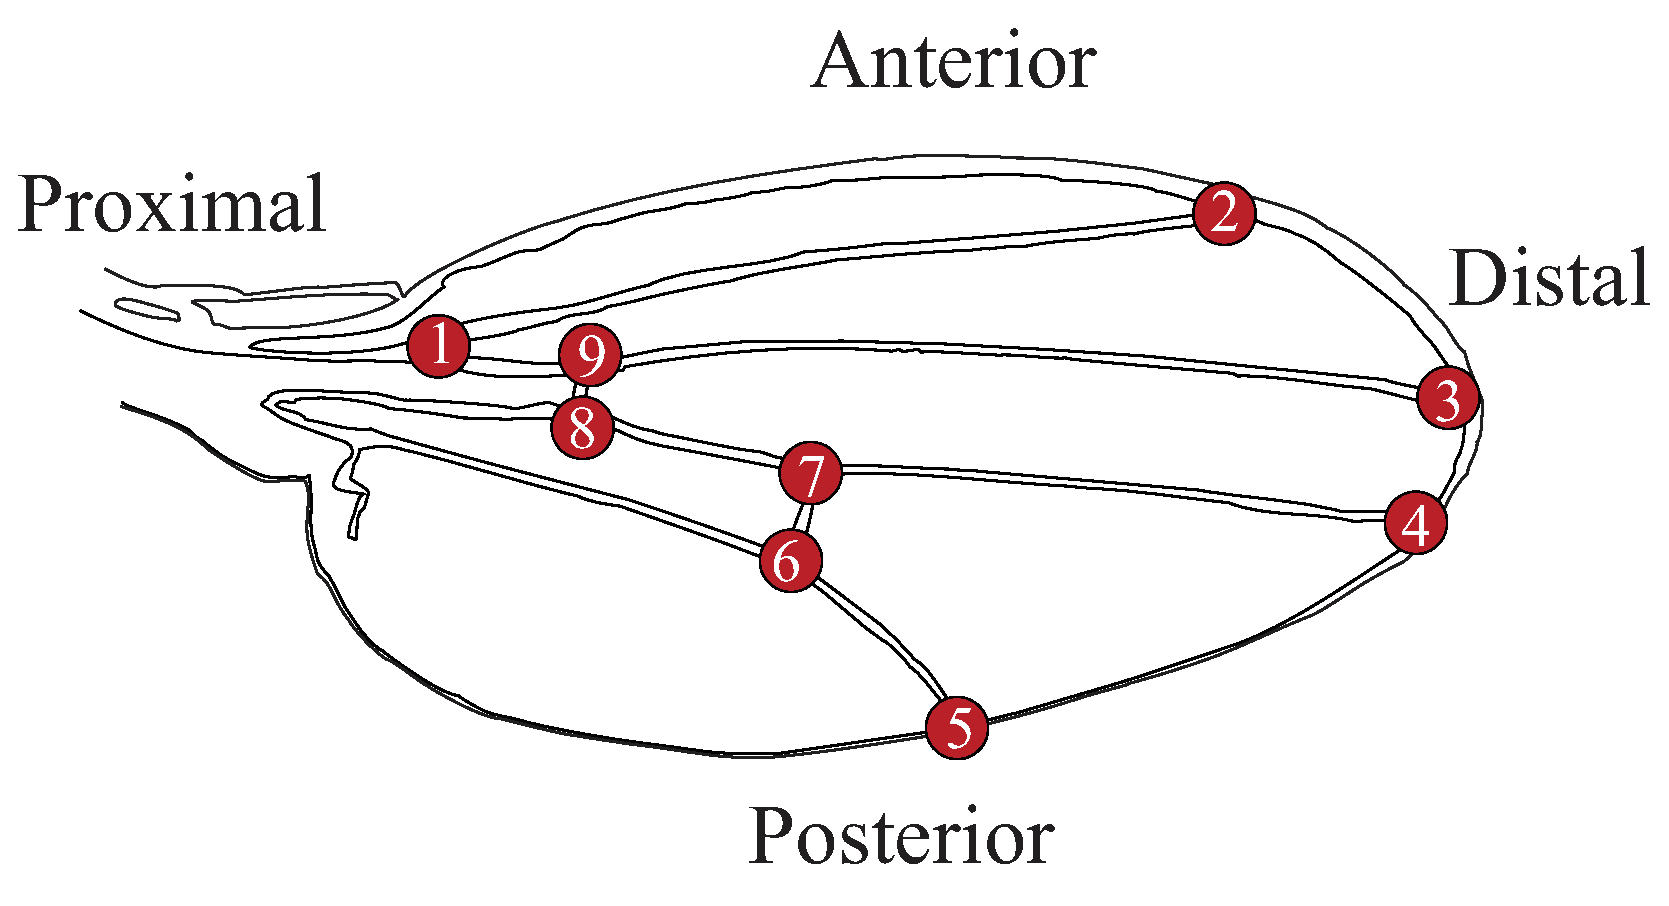
\includegraphics[width=1\textwidth]{WingNineLM}
%\caption{Positions of the nine landmarks used to characterise wing shape.}{Landmarks were: the proximal intersection of the radial vein (1), distal intersection of the radial vein (2), distal intersection of the medial vein (3), distal intersection of the cubital vein (4), distal intersection of the distal vein (5), the posterior (6) and the anterior (7) intersections of the posterior cross vein, and the posterior (8) and the anterior (9) intersections of the anterior cross-vein. Ten interlandmark distances were calculated from Procrustes aligned residuals, and are defined by their end landmarks, i.e., ILD1.8 is the distance between landmarks 1 and 8. Image taken from \citet{McGu13}.}
%\label{fig:WingNineLM}
%\end{figure}
%\newpage

%%=========== Covtest and VL for the 36 Traits =================
%\FloatBarrier
{\renewcommand{\arraystretch}{1.05}}
\begin{table}[!h]
\caption[Covariance parameters estimates and high correlations counts.]{\textbf{Covariance parameters estimates and high correlations counts.} $N$ Correlations~$>~\left|~0.5~\right|$ refers to the number of times a trait had an absolute correlation coefficient greater than 0.5 in the $36 \times 36$ phenotypic correlation plot (see Figure~\ref{fig:CorMAt_36_ILDs} below). The among line variance $V_{Line}$ was estimated for both the small (S) and large (L) treatments.}
\small
\begin{center}
\begin{tabular}{>{\bfseries}lccS[table-format=1.4]S[table-format=1.4]}
\toprule
Index & Trait & {$N$ Correlations $>\left| 0.5 \right|$} & {S Treatment $V_{Line}$ } & {L Treatment $V_{Line}$ } \\
\midrule
ILD1.2 & 2 & 5 & 0.079* & 0.086*\\
ILD1.3 & 3 & 5 & 0.024* & 0.048*\\
ILD1.4 & 4 & 8 & 0.034* & 0.047*\\
ILD1.5 & 5 & 6 & 0.160* & 0.165*\\
ILD1.6 & 6 & 14 & 0.128* & 0.117*\\
ILD1.7 & 7 & 15 & 0.126* & 0.095*\\
ILD1.8 & 8 & 11 & 0.054* & 0.055*\\
ILD1.9 & 9 & 10 & 0.048* & 0.056*\\
ILD2.3 & 10 & 5 & 0.072* & 0.076*\\
ILD2.4 & 11 & 5 & 0.043* & 0.053*\\
ILD2.5 & 12 & 7 & 0.042* & 0.053*\\
ILD2.6 & 13 & 8 & 0.031* & 0.053*\\
ILD2.7 & 14 & 8 & 0.067* & 0.041*\\
ILD2.8 & 15 & 6 & 0.073* & 0.063*\\
ILD2.9 & 16 & 6 & 0.074* & 0.058*\\
ILD3.4 & 17 & 1 & 0.016 & 0.020*\\
ILD3.5 & 18 & 5 & 0.099* & 0.075*\\
ILD3.6 & 19 & 11 & 0.182* & 0.173*\\
ILD3.7 & 20 & 10 & 0.117* & 0.127*\\
ILD3.8 & 21 & 6 & 0.072* & 0.071*\\
ILD3.9 & 22 & 7 & 0.064* & 0.069*\\
ILD4.5 & 23 & 3 & 0.074* & 0.075*\\
ILD4.6 & 24 & 11 & 0.126* & 0.106*\\
ILD4.7 & 25 & 10 & 0.099* & 0.074*\\
ILD4.8 & 26 & 7 & 0.036* & 0.052*\\
ILD4.9 & 27 & 7 & 0.018 & 0.046*\\
ILD5.6 & 28 & 3 & 0.036* & 0.059*\\
ILD5.7 & 29 & 3 & 0.031* & 0.043*\\
ILD5.8 & 30 & 5 & 0.166* & 0.166*\\
ILD5.9 & 31 & 5 & 0.140* & 0.143*\\
ILD6.7 & 32 & 2 & 0.020 & 0.028*\\
ILD6.8 & 33 & 11 & 0.106* & 0.118*\\
ILD6.9 & 34 & 13 & 0.090* & 0.093*\\
ILD7.8 & 35 & 11 & 0.093* & 0.099*\\
ILD7.9 & 36 & 11 & 0.086* & 0.088*\\
ILD8.9 & 37 & 1 & 0.018 & 0.013\\*
\bottomrule
\multicolumn{5}{l}{* indicates significance where $H_0$; $V_{Line}$ = 0, where the probabilty of $\chi^{2}$ was $\leq 0.05$}\\
\end{tabular}
\end{center}
\label{tab:CovTest}
\end{table}
\vspace{-35pt}

\FloatBarrier

%%===========The inital correlation matrix with all 36 ILDs and CS =================
\begin{figure}[htp]
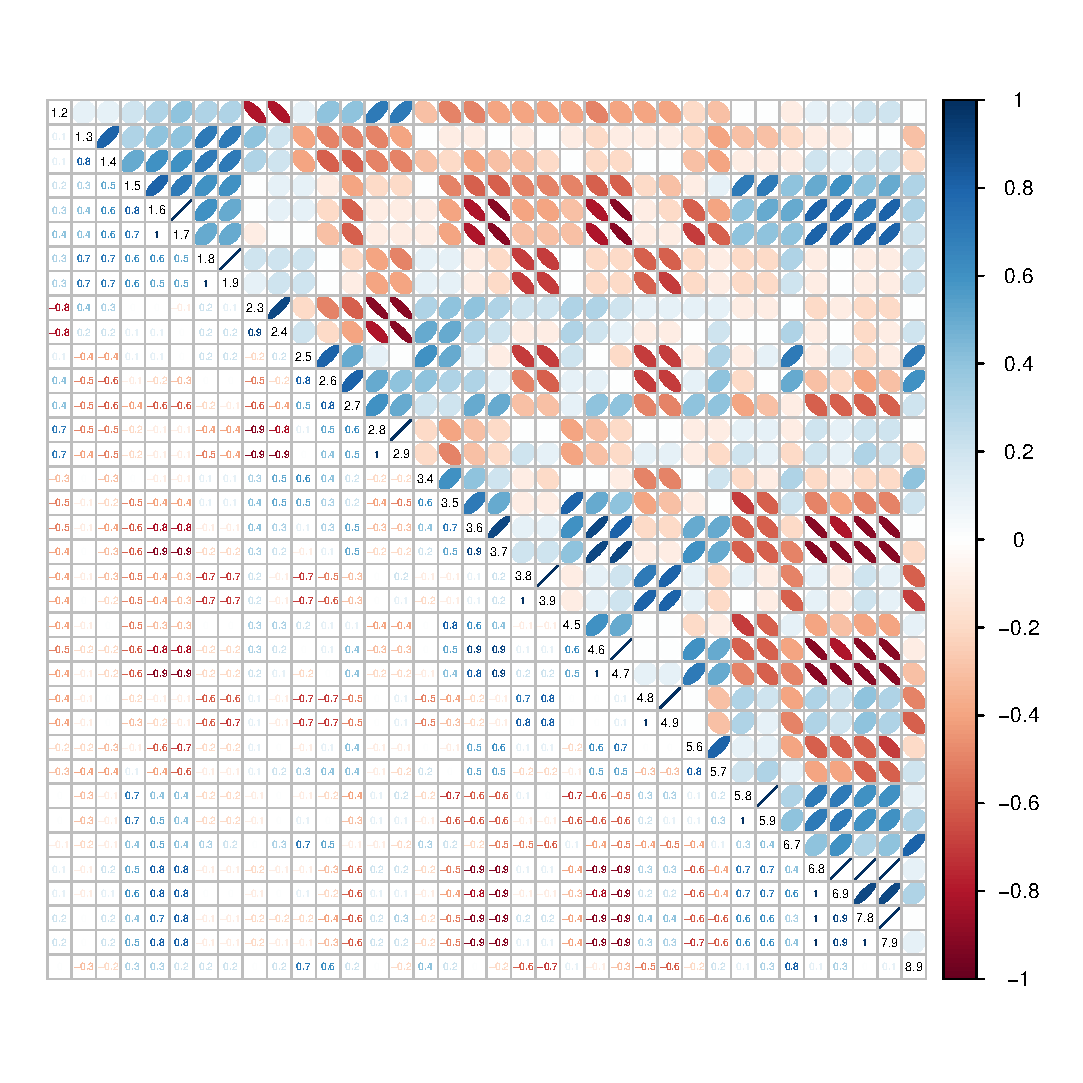
\includegraphics[width=1\textwidth]{Supp/Additional_Info/CorMAt_36_ILDs.eps}
\vspace{-1cm}
\caption[P correlation matrix for 36 inter-landmark distances (ILDs).]
{\textbf{P correlation matrix for 36 inter-landmark distances (ILDs).} Pearson product moment correlations were calculated across the total dataset. The lower off-diagonal is the numerical value. The upper off-diagonal is a schematic representation of the correlation coefficient between two traits, and are shaded as per the legend where blue indicates a positive relationship whereas red indicates a negative relationship. Matrix plot generated using the \textit{corrplot} package in R \citep{corrplot2017}.}
\label{fig:CorMAt_36_ILDs}
\end{figure}
\FloatBarrier
\newpage


%%===========The final wing ILDs and wing coverage =================

\captionsetup[figure]{position=top}
\begin{figure}[!tbp]
  \centering
\subfloat[]{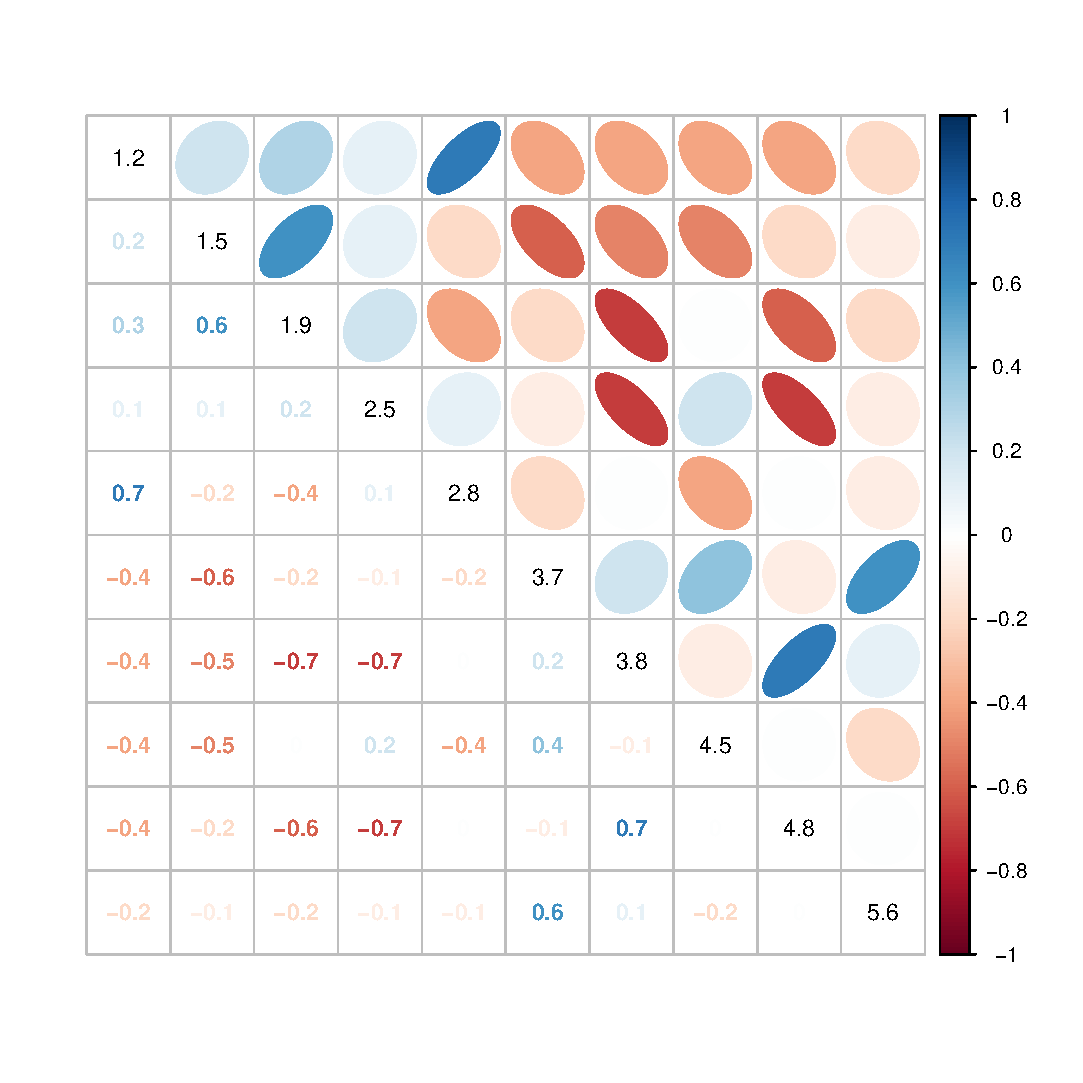
\includegraphics[width=0.8\textwidth]{Supp/Additional_Info/CorMAt_final_ILDs.eps}\label{fig:final_pcorrmat}}
\qquad
   \subfloat[]{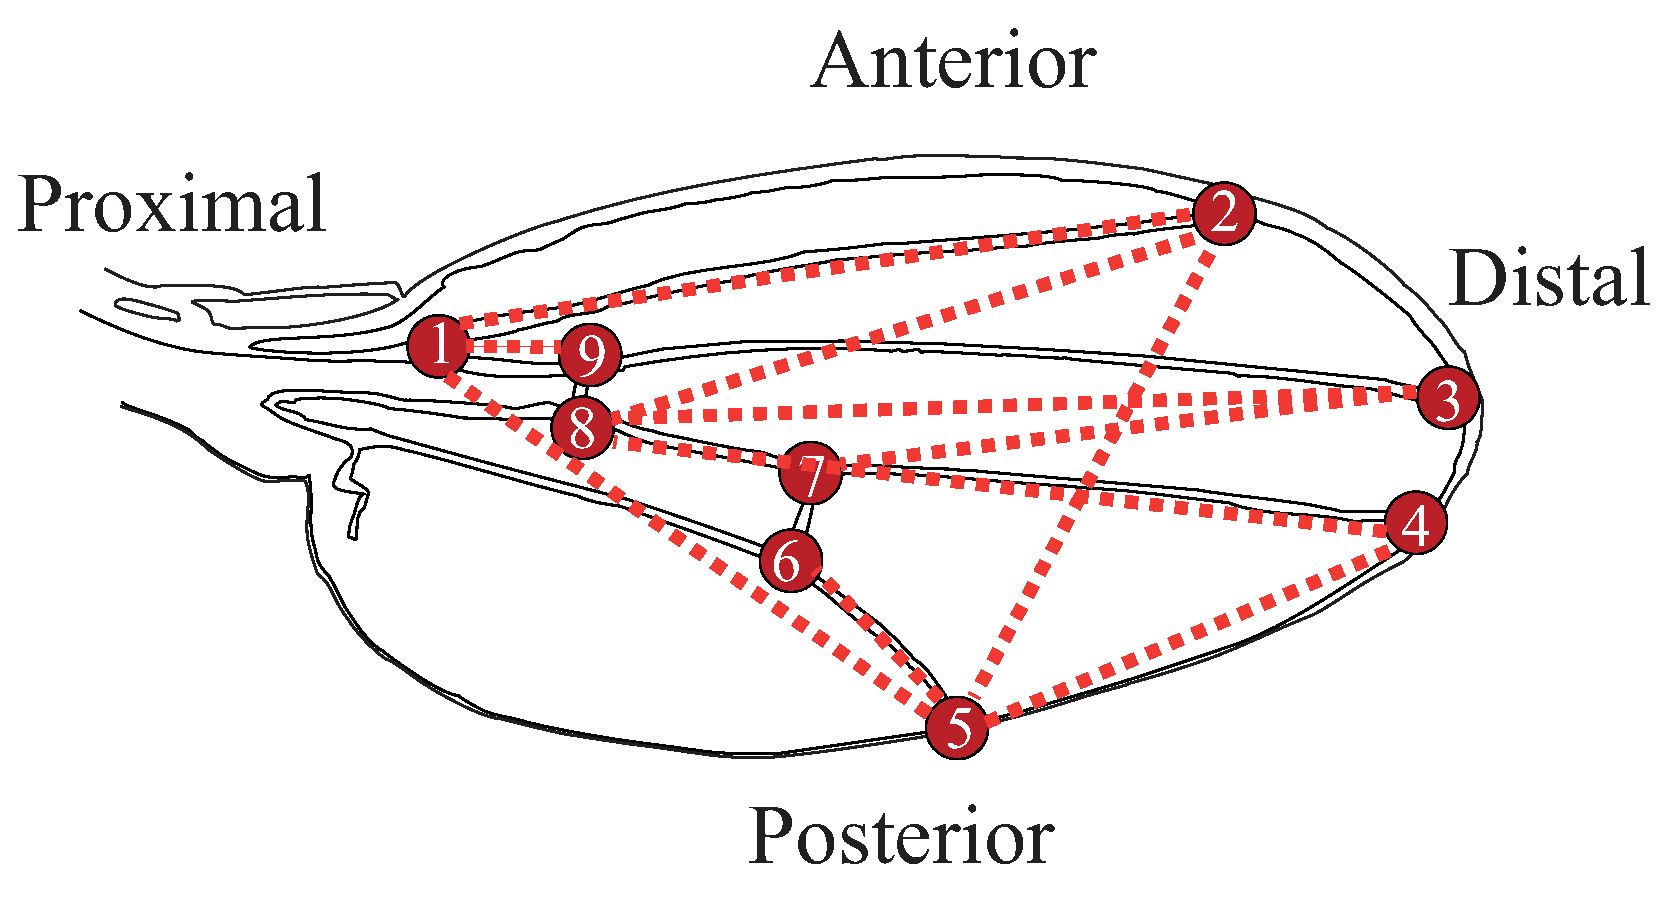
\includegraphics[width=0.7\textwidth]{Supp/Additional_Info/WingNineLM_withILds.eps}\label{fig:final_wingILD}}
  \caption[The P correlation matrix (a) and wing locale (b) for the final 10 ILDs.]{\textbf{The P correlation matrix (a) and wing locale (b) for the final 10 ILDs.} For panel (a) see the above description from Figure~\ref{fig:CorMAt_36_ILDs}. For panel (b),  main text: Figure~\ref{fig:Fig2MetMRdsgn} has been edited to highlight the new inter-landmark distances. The final ten inter-landmark distances selected for \textit{D. serrata} wings are: ILD1.2, ILD1.5, ILD1.9, ILD2.5, ILD2.8, ILD3.7, ILD3.8, ILD4.5, ILD4.8, and ILD5.6. }
\end{figure}


%%=========== Scree plot for eigenanalysis of P =================

%\begin{figure}[htp]
%\includegraphics[width=1\textwidth]{EigenVal_P_36ILDs}
%\vspace{-1cm}
%\caption{Scree plot for P cov}{xx}
%\label{fig:eigP}
%\end{figure}
%\FloatBarrier
%\newpage




